% Prvi del predavanja: nasveti 1–3 in utesnjena prosojnica nasveta 4, v temi
% Berlin in razmerju 4 : 3. Predavanje se začne kot slabo predavanje in
% popravlja po eno težavo naenkrat; vsak popravek pokaže naslednjo težavo. Vsak
% nasvet ima kratko prosojnico s kodo. O razdelitvi na tri dokumente glej
% stevilke.tex.
\documentclass{beamer}
\usepackage[utf8]{inputenc}
\usepackage[T1]{fontenc}
\usepackage[slovene]{babel}
\usepackage{amsmath}
\usepackage{minted}
\usepackage{tikz}
\usetikzlibrary{decorations.pathreplacing}
\usetheme{Berlin}
% Predavanje je razdeljeno na tri dokumente, ker se tema in razmerje sredi
% dokumenta ne dasta zamenjati: berlin-4-3.tex, berlin-16-9.tex in
% prosojnice.tex, ki prva dva vključi. Številke prosojnic se nadaljujejo iz
% dokumenta v dokument: ob koncu dokument zapiše zadnjo številko v datoteko
% ⟨ime⟩.stevec, naslednji pa jo prebere z \input{⟨ime⟩.stevec}. Dokumente zato
% prevajajte po vrsti.
\makeatletter
\AtEndDocument{%
  \newwrite\stevec
  \immediate\openout\stevec=\jobname.stevec
  \immediate\write\stevec{\string\setcounter{framenumber}{\the\c@framenumber}}%
  \immediate\closeout\stevec
}
\makeatother


\newcommand{\ukaz}[1]{\texttt{\textbackslash#1}}

% Majhna prosojnica s tremi vrsticami za sliko o \only in \onslide. Prvi
% argument je središče, drugi vsebina, ki jo narišemo vanjo.
\newcommand{\mala}[2]{%
  \begin{scope}[shift={#1}]
    \draw[gray] (-0.8, -0.7) rectangle (0.8, 0.7);
    #2
  \end{scope}%
}

\AtBeginSection{
  \begin{frame}
    \sectionpage
  \end{frame}
}

\title{Predstavitve}
\author{Računalniški praktikum}
\date{18.~november~2026}

\begin{document}

\begin{frame}
  \titlepage
\end{frame}

\section{Ne berite prosojnic}

% Predavatelj prosojnico prebere na glas, besedo za besedo. Besedilo namenoma
% sega čez spodnji rob.
\begin{frame}{Ne berite prosojnic}
  Prosojnice niso namenjene temu, da bi nanje zapisali vse, kar
  povemo, temveč temu, da predavatelju pomagajo pokazati tisto, kar je
  lažje razložiti s sliko kot z besedami. Idealna prosojnica je zato
  prazna, vsaka stvar na njej pa si mora svoje mesto prislužiti s tem,
  da pokaže nekaj, kar je težko povedati. Besedilo, ki ga poslušalci
  lahko preberejo sami, sodi v zapiske ali učbenik, ne na prosojnico.
  Če prosojnica le ponovi tisto, kar predavatelj tako ali tako pove,
  poslušalcem odvrača pozornost, saj ne vedo, ali naj berejo ali
  poslušajo. Še več, poslušalci berejo hitreje od predavatelja, zato
  do konca besedila pridejo pred njim in začnejo razmišljati o drugih
  stvareh.
\end{frame}

\section{Osredotočite se na eno stvar}

% Predavatelj te prosojnice ne bere.
\begin{frame}{Zakaj?}
  \begin{itemize}
    \item poslušalci vedo, na kaj naj bodo pozorni
    \item na prosojnici je več prostora, da pokažemo idejo
    \item poslušalci vas prehitijo in nehajo poslušati
    \item eno samo idejo lahko smiselno povzamete v naslovu
    \item v Beamerju novo prosojnico naredimo z okoljem \texttt{frame}
    \item Beamer zna vsebino razkrivati po korakih
  \end{itemize}
\end{frame}

% Slaba prosojnica naslednjega nasveta: možnosti, opisane z besedami.
\begin{frame}{Beamer razkriva vsebino na več načinov}
  \begin{itemize}[<+->]
    \item Ukaz \ukaz{only<2>\{\dots\}} vsebino prikaže samo na drugem koraku, na
      ostalih korakih pa je ni in ne zaseda prostora.
    \item Ukaz \ukaz{onslide<2>\{\dots\}} vsebino na ostalih korakih skrije,
      prostor zanjo pa ostane.
    \item Ukaz \ukaz{alert<2>\{\dots\}} vsebino na drugem koraku poudari, na
      ostalih pa jo prikaže kot običajno besedilo.
    \item Ukaz \ukaz{invisible<2>\{\dots\}} vsebino skrije samo na drugem koraku,
      prostor zanjo pa ostane.
  \end{itemize}
\end{frame}

\section{Slika je vredna več kot tisoč besed}

% Slika se gradi po korakih. Ukaz \only spremeni velikost slike, zato je meja
% slike določena vnaprej.
\begin{frame}{Beamer razkriva vsebino na več načinov}
  \centering
  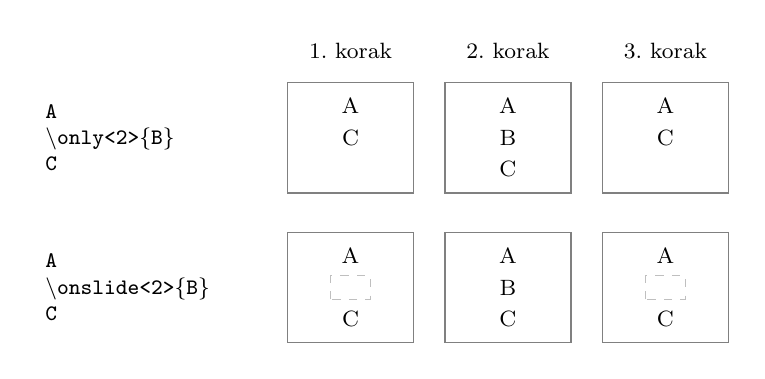
\begin{tikzpicture}[font=\footnotesize]
    \useasboundingbox (-0.1, -2.7) rectangle (8.9, 1.4);
    \foreach \k in {1, 2, 3} {
      \node at (2 + 2 * \k, 1.1) {\k.\ korak};
    }
    \node[anchor=west, align=left, font=\ttfamily\footnotesize] at (0, 0)
      {A\\\textbackslash only<2>\{B\}\\C};
    \mala{(4, 0)}{\node at (0, 0.4) {A}; \node at (0, 0) {C};}
    \mala{(6, 0)}{\node at (0, 0.4) {A}; \node at (0, 0) {B}; \node at (0, -0.4) {C};}
    \mala{(8, 0)}{\node at (0, 0.4) {A}; \node at (0, 0) {C};}
    \only<2->{
      \node[anchor=west, align=left, font=\ttfamily\footnotesize] at (0, -1.9)
        {A\\\textbackslash onslide<2>\{B\}\\C};
      \mala{(4, -1.9)}{\node at (0, 0.4) {A}; \draw[gray!50, dashed] (-0.25, -0.15) rectangle (0.25, 0.15); \node at (0, -0.4) {C};}
      \mala{(6, -1.9)}{\node at (0, 0.4) {A}; \node at (0, 0) {B}; \node at (0, -0.4) {C};}
      \mala{(8, -1.9)}{\node at (0, 0.4) {A}; \draw[gray!50, dashed] (-0.25, -0.15) rectangle (0.25, 0.15); \node at (0, -0.4) {C};}
    }
  \end{tikzpicture}
\end{frame}

% V razmerju 4 : 3 sta dokaza utesnjena; to vodi v širok format.
\newcommand{\vsotakoraki}{1-}
% Dva dokaza formule za vsoto prvih n števil. Prosojnico vključita
% berlin-4-3.tex, kjer je utesnjena, in berlin-16-9.tex, kjer je najprej še z
% glavo in nogo, nato pa brez njiju. Dokument mora naložiti paketa amsmath in
% tikz s knjižnico decorations.pathreplacing ter z ukazom \vsotakoraki določiti,
% katere korake prosojnice pokaže: v berlin-4-3.tex vse (1-), v
% berlin-16-9.tex le zadnjega (4), saj se tam slika ne gradi več.
\begin{frame}<\vsotakoraki>{V matematiki so slike sploh pomembne}
  \begin{columns}[T]
    \begin{column}{0.48\textwidth}
      \begin{block}{Indukcija}
        \scriptsize
        % Razmik okoli izpeljave ostane sicer takšen kot pri običajni velikosti.
        \setlength{\abovedisplayskip}{3pt}
        \setlength{\belowdisplayskip}{3pt}
        Trdimo, da za vsak \(n \geq 1\) velja
        \(1 + 2 + \dots + n = n(n + 1)/2\).

        \emph{Baza.} Za \(n = 1\) je leva stran \(1\), desna pa
        \(1 \cdot 2/2 = 1\).

        \emph{Korak.} Predpostavimo, da formula velja za \(n\). Po indukcijski
        predpostavki je
        \begin{align*}
          &1 + \dots + n + (n + 1)
          = \frac{n(n + 1)}{2} + (n + 1) \\
          &= \frac{n(n + 1) + 2(n + 1)}{2}
          = \frac{(n + 1)(n + 2)}{2},
        \end{align*}
        kar je formula za \(n + 1\). Po načelu indukcije formula velja za vsak
        \(n \geq 1\).
      \end{block}
    \end{column}
    \begin{column}{0.48\textwidth}
      \begin{block}{Slika}
        \centering
        % Modro stopnišče je 1 + 2 + 3 + 4, rdeče je enako, le obrnjeno. Skupaj
        % dasta pravokotnik n × (n + 1).
        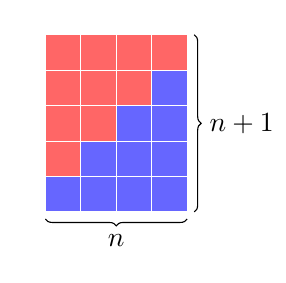
\begin{tikzpicture}[x=0.45cm, y=0.45cm]
          \useasboundingbox (-0.5, -1.2) rectangle (6, 5.2);
          \foreach \i in {1, ..., 4}
            \foreach \j in {1, ..., \i}
              \fill[blue!60, draw=white] (\i - 1, \j - 1) rectangle ++(1, 1);
          \foreach \i in {1, ..., 4}
            \foreach \j in {\i, ..., 4}
              \fill<2->[red!60, draw=white] (\i - 1, \j) rectangle ++(1, 1);
          \draw<3->[decorate, decoration={brace, mirror}] (0, -0.2) -- (4, -0.2)
            node[midway, below=2pt] {\(n\)};
          \draw<3->[decorate, decoration={brace, mirror}] (4.2, 0) -- (4.2, 5)
            node[midway, right=2pt] {\(n + 1\)};
        \end{tikzpicture}

        \onslide<4->{\(2 (1 + \dots + n) = n (n + 1)\)}
      \end{block}
    \end{column}
  \end{columns}
\end{frame}


\end{document}
